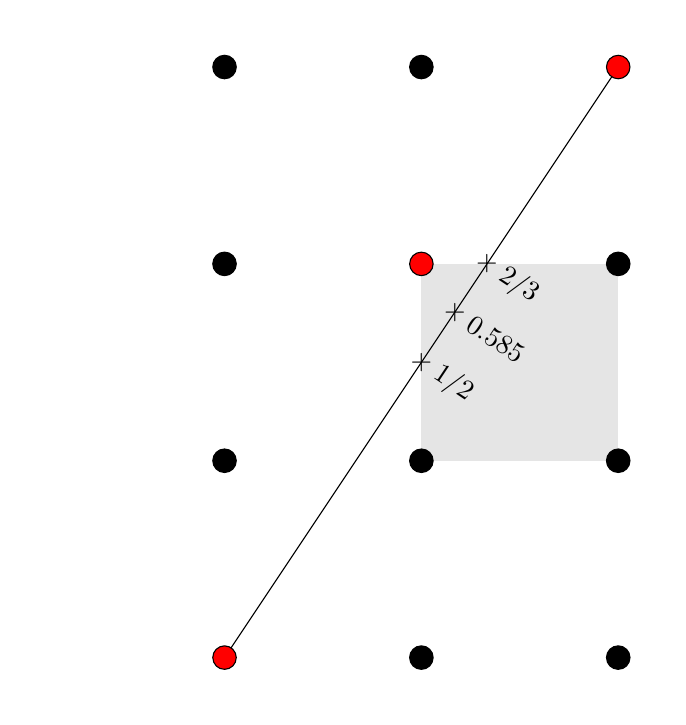
\begin{tikzpicture}[scale=2.5]

\clip (0 - 1, 0 - 0.2) rectangle (2 + 0.2, 3 + 0.2);
\fill[fill=gray!20] (1, 1) rectangle (2, 2);
\draw (0, 0) -- (0 + 2, 0 + 3);
\draw (1, 3/2) node[] {$+$};
\draw (1, 3/2) node[right, rotate=-33.690067525979785] {\;1/2};
\draw (1.17, 1.755) node[] {$+$};
\draw (1.17, 1.755) node[right, rotate=-33.690067525979785] {\;0.585};
\draw (4/3, 2) node[] {$+$};
\draw (4/3, 2) node[right, rotate=-33.690067525979785] {\;2/3};
\draw (0, 0) node[circle,draw=black,fill=red,inner sep=3pt] {};
\draw (0, 1) node[circle,draw=black,fill=black,inner sep=3pt] {};
\draw (0, 2) node[circle,draw=black,fill=black,inner sep=3pt] {};
\draw (0, 3) node[circle,draw=black,fill=black,inner sep=3pt] {};
\draw (1, 0) node[circle,draw=black,fill=black,inner sep=3pt] {};
\draw (1, 1) node[circle,draw=black,fill=black,inner sep=3pt] {};
\draw (1, 2) node[circle,draw=black,fill=red,inner sep=3pt] {};
\draw (1, 3) node[circle,draw=black,fill=black,inner sep=3pt] {};
\draw (2, 0) node[circle,draw=black,fill=black,inner sep=3pt] {};
\draw (2, 1) node[circle,draw=black,fill=black,inner sep=3pt] {};
\draw (2, 2) node[circle,draw=black,fill=black,inner sep=3pt] {};
\draw (2, 3) node[circle,draw=black,fill=red,inner sep=3pt] {};

\end{tikzpicture}
